\section{Busienss Model}\label{business_model}

\paragraph{} In this section we will explain the business model canvas, since Arckane is working on top of two industries we will use labels, in figure \ref{fig:modelcanvas} \textbf{(p)} purple is referencing the education industry, \textbf{(a)} aqua is referencing the recruiting industry and \textbf{(y)} yellow is referencing general Arckane activities. Self explanatory topics will just be listed.

% SUBSECTION: Value Proposition

\subsection{Value Proposition}\label{valueproposition}

\paragraph{(p) Easily find and pay for tailor made education:} Finding tutors and paying them is as easy as doing a couple of taps in the app. As described in section \ref{justification} the distributed education system enables tutors to have deep knowledge of the status of their apprentices. 1) They can directly see in the ontology what is the proficiency of all the specific skills of the apprentice, making placement exams unnecessary. 2) The results of the research on education enables us to create apprentice profiles (what they are more stimulated with, what are the techniques that have worked the best with them, etc.) and this profile is improved over time with help of the tutors. Also machine learning can be used to make Arckane learn how apprentices learn, making an automatic recommendation system of the best resources and tutors that suit the apprentice learning styles. 

\paragraph{(p) Easily offer and charge for teaching any skill:} It is easy to offer tutoring through Arckane thanks to the automatic scheduling system, all you have to do as a tutor is tell Arckane your free times and wait for new apprentices to come. Also receiving payments is easy because Arckane charges the apprentices beforehand, tutors have nothing to worry about charging. Also Arckane can recommend the tutor how much to charge for different skills since in the system we know the offer and demand of tutoring for all the skills.

\paragraph{(p) Education becomes cheaper:} The factors that will lower the education price are: 1) There are no institutions with bureaucracy involved. 2) The system automates logistics. 3) The tutoring market is digitalized, so working and studying the economy characteristics is faster, easier, better and some time automatic. 4) Combined with the digital skill market we can transform education into education on demand, people can develop ONLY the skills they need, and do not have to waste valuable resources (money and time) on skills they may never use.

\paragraph{(p) Arckane is dedicated to making you an amazing tutor:} Since we are creating an automated digital system with a very good business model Arckane can use its efforts and resources in researching education, studying the distributed education system fenomenas and bringing new knowledge, tools and techniques to the tutors, this value is given to every tutor in the world, giving massive reach to education research. 

\paragraph{(a) Instantly find talent:} Since Arckane has a complete, objective, certified and granular database of the skills the apprentices process (with levels of proficiency) we can offer a search engine for talent which perfectly matches the needs of the query, one may search sets of skills with different proficiencies and other criteria like geolocation. This creates an open digitalized skill market, where anyone can find talent, from a plumber, a cook, or a software engineer.

\paragraph{(a) Organizations save a lot of money, time and resources in recruiting:} Last proposition value also applies to companies, we can offer reliable automatic talent matchmaking that satisfy the necessities of the company. Also companies can post job skill sets, a publication of what are the skill profiles they are looking for in different positions, then apprentices can work in creating those skills and achieving the level of proficiency needed, this way we can also convert education into education on demand.

\paragraph{(a) Automatically find job for any of your skills:} Any apprentice can offer their skills in the skill market, which can be constantly be looking for projects or jobs for them, from freelance projects, research groups or long term jobs.

\paragraph{(a) Get rating of your skills by organizations:} When an apprentice has been employed the organization can rate new levels of proficiency and newly obtained skills, this way apprentices can reflect their improvements to the system by working or participating in projects.

\paragraph{(a) Organizations can attract employees using the reputation system:} Organizations gain reputation when they rate their employees skills, reputation that reflects how much employees can improve when working in the organization (and on which skills). Also organizations can build in this way a profile of the skills currently being used inside the organization.

% SUBSECTION: Customer Segments

\subsection{Customer Segments}

\paragraph{(p) Any person who wants to learn something}

\paragraph{(p) Any person who wants to teach something:} And/or wants to create economic opportunities for himself by teaching and transferring his skills.

\paragraph{(a) Any person who wants to sell their skill services:} And/or is looking for an interesting project or job in which he can use their skills.

\paragraph{(a) Any person looking for someone with a skill:} Or even specific skill sets.

\paragraph{(a) Organizations looking for talent automatically:} And specially organizations who want to massively cut costs in recruiting.

% SUBSECTION: Revenue Streams

\subsection{Revenue Streams}

\paragraph{(p) Apprentice fee:} Each time a session is paid Arckane charges a fee to the apprentice which may vary from 5\% to 15\%.

\paragraph{(a) Freelance employer fee:} Each time someone is paid for their skills through the digital skill market Arckane charges a fee to the employer which may vary from 5\% to 15\%.

\paragraph{(a) Recruiting fee:} Arckane charges organizations a fee for the matchmaking of talent, this specific business model is still under consideration, considered options for now are monthly fee or per contract fee.

% SUBSECTION: Cost Structure

\subsection{Cost Structure}

\paragraph{(y) Software development}

\paragraph{(y) Deployment cloud services}

\paragraph{(p) Education research}

\paragraph{(y) Logistic employees}

\paragraph{(y) Customer care}

% SUBSECTION: Key Activities

\subsection{Key Activities}\label{keyactivities}

\paragraph{(p) Software development of the distributed education system:} The app interfaces, scheduling system, payments, communications, etc.

\paragraph{(p) Research in education:} As mentioned in the value proposition \ref{valueproposition} subsection to achieve high quality custom education Arckane must research the state of the art of education and do improvements in the field, this will highly increase the whole value of the distributed education system and of Arckane overall.

\paragraph{(p) Offer tutors tools and knowledge:} See last key activity.

\paragraph{(a) Software development of the digital skill market}

\paragraph{(y) Customer care}

% SUBSECTION: Key Resources

\subsection{Key Resources}\label{keyresources}

\paragraph{(y) Cloud services providers}

\paragraph{(y) Founding}

\paragraph{(p) Alliances with schools and online courses:} One important aspect of the distributed education system is that it does NOT fight or goes against the current systems, to follow the mission of the corporation we can open an API so that people certify and rate their skills in Arckane also through the traditional system and the online courses services, giving more value to the skills developed through these systems and creating a stronger digital market of skills for Arckane.

% SUBSECTION: Key Partners

\subsection{Key Partners}

\paragraph{Large companies constantly looking for talent:} Large companies invest large amounts of resources into recruiting, with strong partnerships Arckane can extremely lower their investment into recruitment with more efficient and effective results.

\paragraph{Schools, universities and online courses companies:} As mentioned in the Key Resources \ref{keyresources} subsection, Arckane can create strong partnerships with the service providers of the other education systems to give more value to their certifications and create a stronger digital skills market.

\paragraph{Education research groups:} As mentioned in the Key Activities \ref{keyactivities} subsection, it is of extreme importance for Arckane to be an important agent in the education research field, for this partnerships with research groups around the globe will be of much benefit.

% SUBSECTION: Customer Relationships

\subsection{Customer Relationships}

\paragraph{} All topics of this subsection are mentioned in the \ref{growthplan} Growth Plan section.

% SUBSECTION: Channels

\subsection{Channels}

\paragraph{(y) App stores:} Which have rating systems where we can interact with customers which have rated the app.

\paragraph{(y) Web:} Through the app and the help tools.

\paragraph{(y) Call center}

\paragraph{(p) Events:} Like the Arckane Fairs (see section \ref{growthplan})

% Business model figure
\pagebreak
\newgeometry{top=1.5in,bottom=1in,right=0in,left=0in} % Change page margins
\begin{figure}[h] % Figure
    \centering
    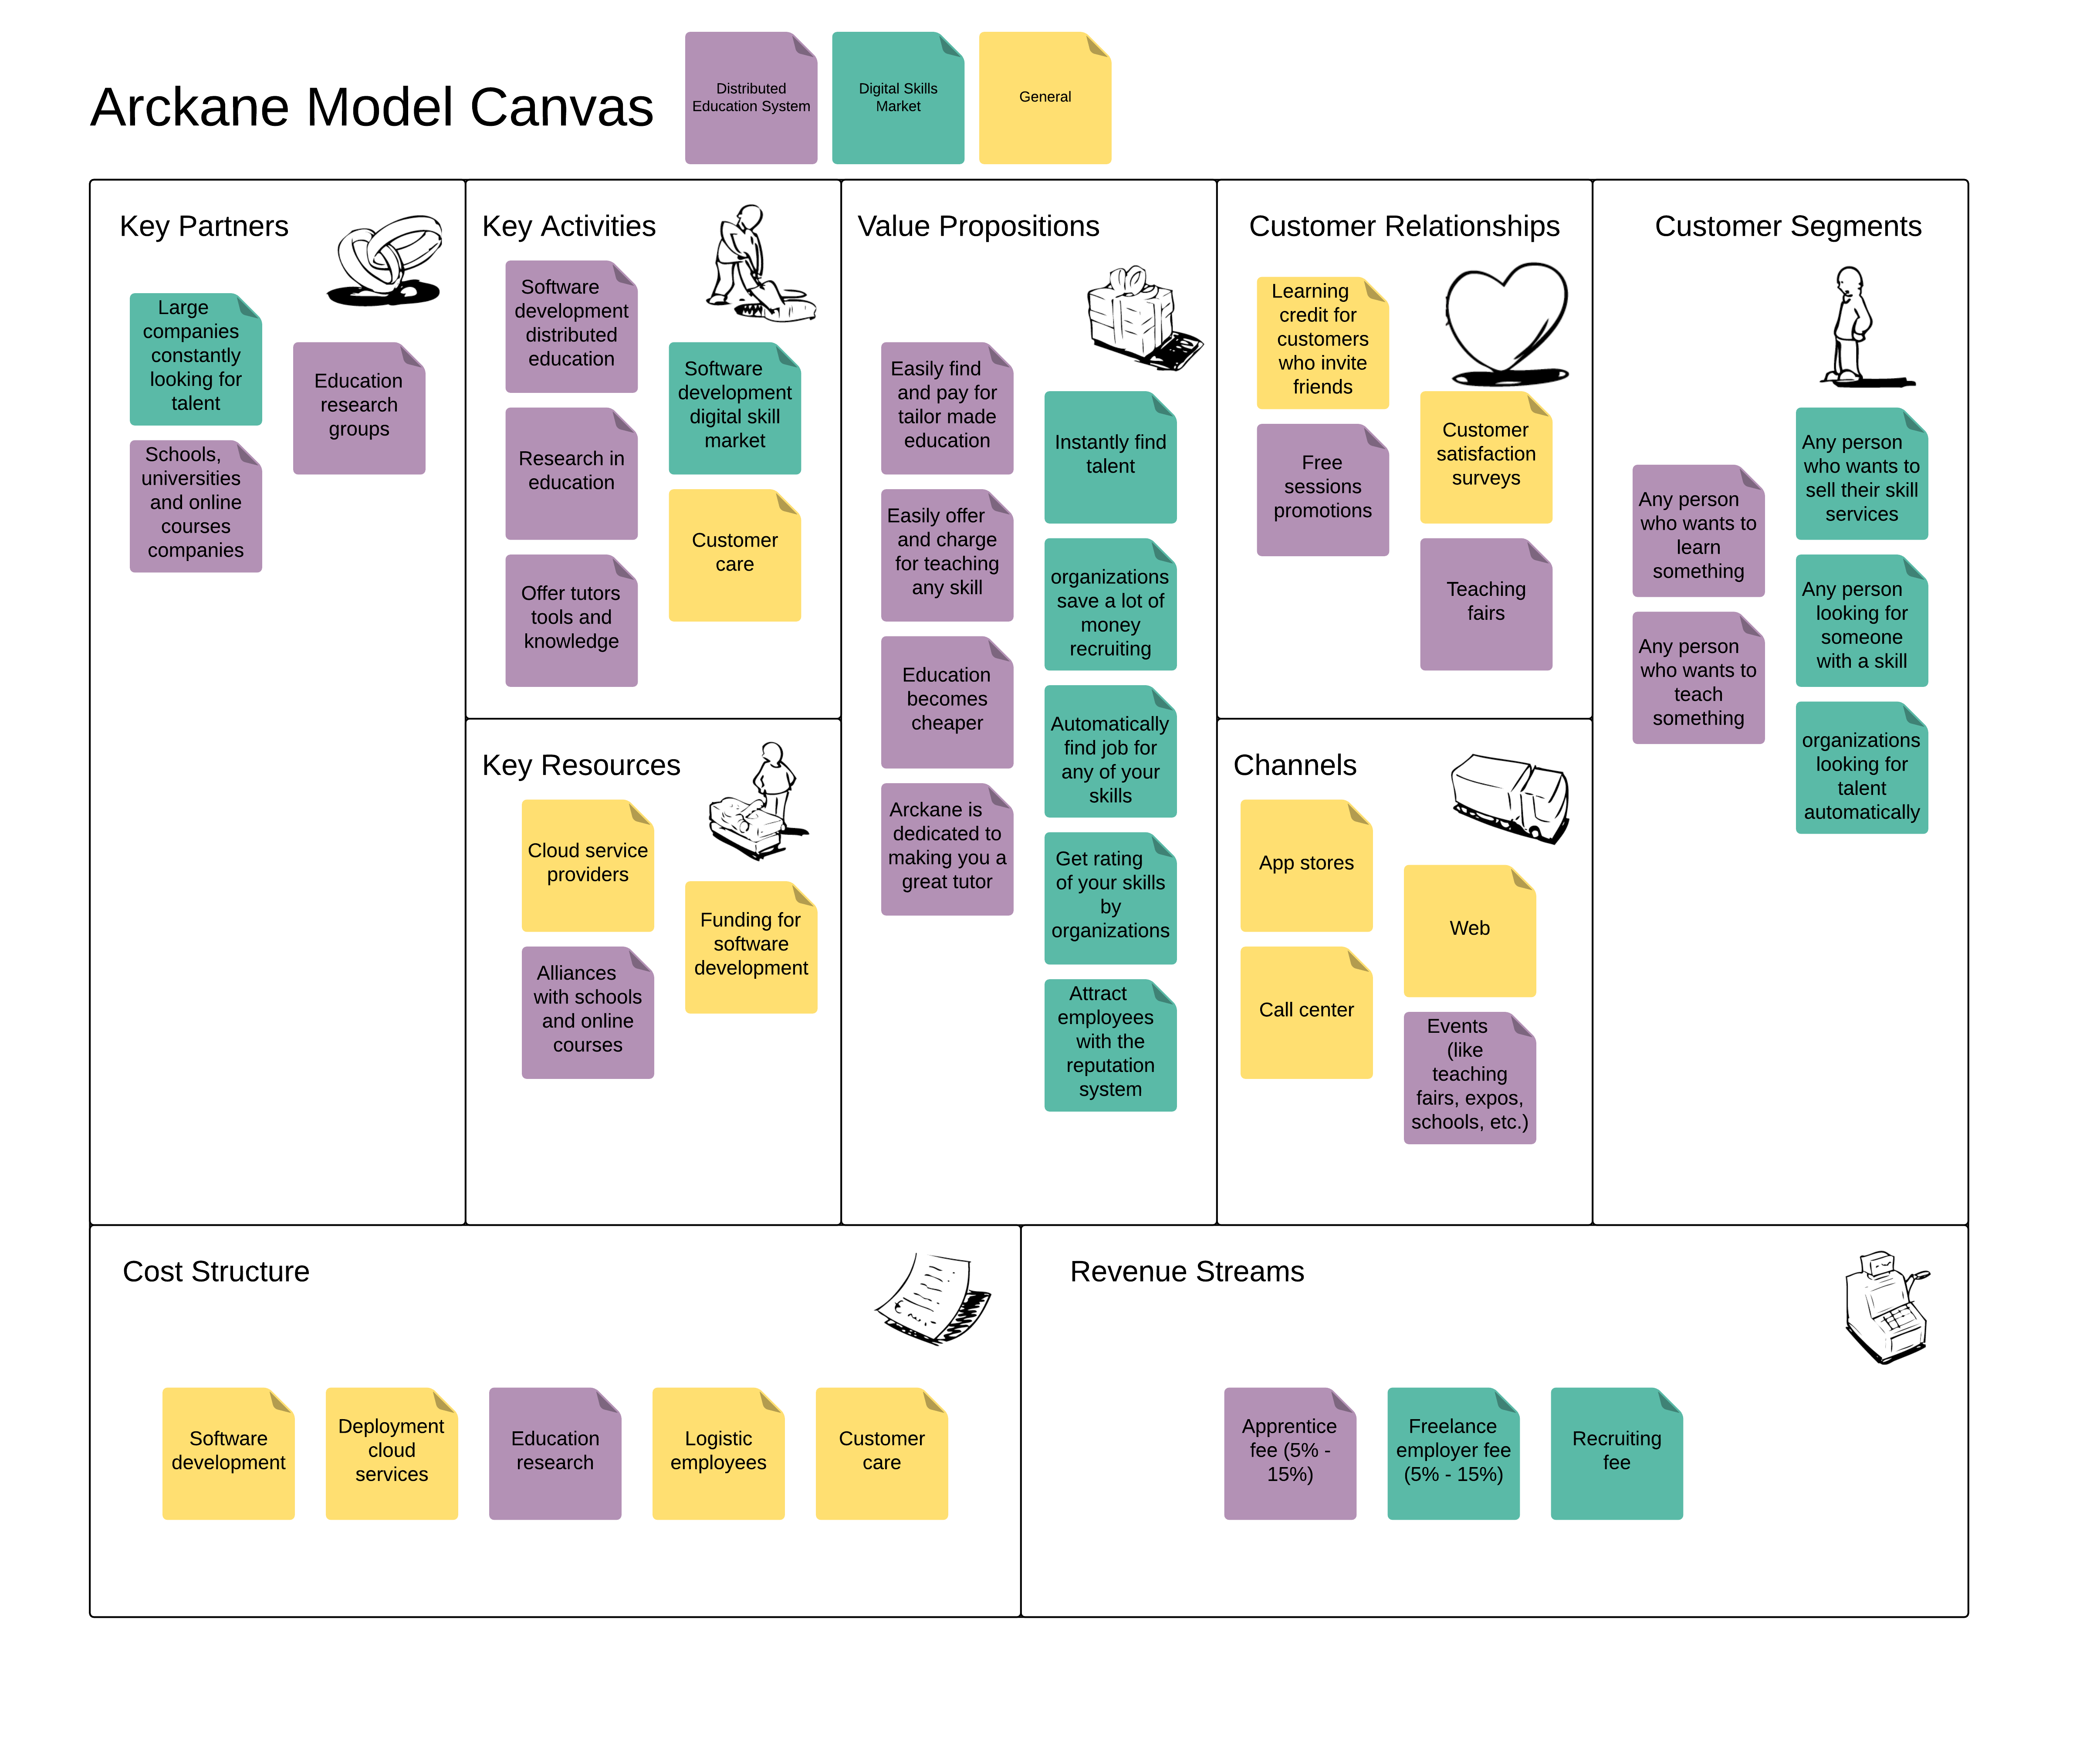
\includegraphics[width=\textwidth]{modelcanvas}
    \caption{Arckane Business Model Canvas}
    \label{fig:modelcanvas}
\end{figure}
\restoregeometry % Restore page margins
\pagebreak